\section{Rectification test}

The following test was performed to verify the correctness of the pixel
associations with respect to the rectified images given by \textit{image\_proc}
of \texttt{ROS}.
The difference of intensities at corresponding pixels in the original images $I_{j}$ and rectified images $I_{j}^{rect}$ are given by:

\begin{equation}
  \Delta I_{i,j} = I_j(u_{i,j}) - I_j^{rect}(w_{i,j}) 
  \hspace{1em} \text{for } i = 1 \ldots n \text{, } \hspace{1em} j = 1,2
  \hspace{1em}\text{,}
  \label{eqn:rect/I_def}
\end{equation}

where $u_{i,j}$, $w_{i,j}$ denote the pixel location of the object point $X_i$ in the
original and rectified image of camera $j$ respectively.

If the rectified pixels are computed in accordance with the rectification
process given by \texttt{ROS}, this difference should be
approximately zero or

\begin{equation}
  I_j(u_{i,j}) = I_j^{rect}(w_{i,j}) + \epsilon_{i,j} 
  \hspace{1em} \text{for } i = 1 \ldots n \text{, } \hspace{1em} j = 1,2
  \hspace{1em}\text{,}
  \label{eqn:rect/diffI_eq}
\end{equation}

with the error $\epsilon_{i,j}$ arising solely from interpolation.

The pixels of the rectified images are computed using the projection matrices
$P_{j} = K' \begin{bmatrix} I | t_j \end{bmatrix}$ and rotation matrices $R_j$ 
obtained from the \textit{CameraInfo} message with \cite{WikiCameraInfo}

\begin{align}
  w_{i,j} &= K'(R_j T_j(X_i)) \hspace{1em} \text{, where} \\
  T_j(X_i) &= \pi(_{C_j}r_{C_jX_i}) \\
           &= \pi(C_{C_j M} (X_i - {_M}r_{MC_j})) \hspace{1em} \text{and} \\
  \pi(\begin{pmatrix} x, y, z \end{pmatrix}^T) &= 
  \begin{pmatrix} x/z, y/z, 1 \end{pmatrix}^T 
  \hspace{1em}\text{.}
  \label{eqn:rect/utilde_def}
\end{align}

The parameters related to the pose of each camera are obtained from

\begin{align}
  C_{C_jM} &= C_{C_jS} C_{SM} = R_j^TC_{SM} \hspace{1em} \text{and} \\
  _{M}r_{MC_j} &= C_{MS}(_{S}r_{SC_j} - _{S}r_{SM}) \\
  &= C_{MS}(-t_j - _{S}r_{SCM})\hspace{1em} \text{.}
\end{align}

The pose of the stereo frame with respect to the map frame ($C_{MS}$, $_{M}r_{MS}$) is estimated such that all map
point projections lie inside both images.

The last information missing for calculating the pixel correspondences are 
the distorted pixels which are simply given by 

\begin{equation}
  u_{i,j} = K_j D_j(T_j(X_i))) 
  \hspace{1em} \text{for } i = 1 \ldots n \text{, } \hspace{1em} j = 1,2
  \hspace{1em}\text{,}
  \label{eqn/rect/u_def}
\end{equation}

with $K_j$ and $D_j$ the camera matrix and distortion function and $T_j$ the same
projection function as given above. 

A look at Figures \ref{fig:rect_r1} and \ref{fig:rect_r2} shows that the resulting error
between the rectified image and the original image is indeed uniformly 
small and with only very light patterns observable in both left and right images.
These patterns get stronger as we approach the image border, where interpolation
effects become more important.
The pixel correspondence equations developed above are thereby validated for the 
rectified images provided by \textit{image\_proc}.

\newpage
\section{Transformation test}

Similar considerations can be applied for validating the interpretation of the
camera parameters to compute the transformation between the left and the right
camera.

The following assumptions need to be tested \cite{DocCameraInfo},
\cite[p. 523f]{Siciliano2007}.

\begin{equation}
  C_{SC_j} = R_j \hspace{1em} \text{and} \hspace{1em} _{S}r_{SC_j} = -t_j 
  \hspace{1em}\text{for j=1,2} \hspace{1em} \text{.}
  \label{rect/eqn:assumptions}
\end{equation}

If the above assumptions hold, then one can obtain the point coordinates in the second camera frame from the
ones in the first camera frame by applying

\begin{align}
  _{C_2}r_{C_2X_i} &= C_{C_2C_1} (_{C_1}r_{C_1X_i} + _{C_1}r_{C_1C_2}) 
  \hspace{1em} \text{for } i = 1 \ldots n \text{, with} \\ 
  C_{C_2C_1} &= R_2^TR_1 \hspace{1em} \text{and} \\
  _{C_1}r_{C_1C_2} &= C_{C_1 S} (_S{r}_{S C_2} - _S{r}_{S C_1}) \\
  &= R_1^T (t_1 - t_2)
  \hspace{1em} \text{.} 
\end{align}

The same transformations as before are then applied to project these points in
the respective rectified images. 

As can be seen from Figure \ref{fig:rect_r2_transform}, the resulting
intensity difference image is identical with the one from the preceding
procedure where the pixels were
directly projected from the world frame to the left and right image (Figure
\ref{fig:rect_r2}). 
Therefore, the transform between the left and right image is computed correctly.
\textit{No! This only tells me that I was consistent with my transformations and
not that the transformations are indeed right\ldots (Check with examples with
correct depth information if the transformations are right.)}

\begin{figure}[h]
  \centering
  \begin{subfigure}[b]{0.7\textwidth}
    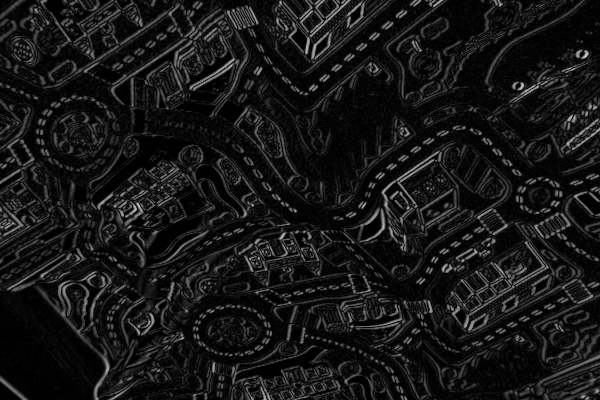
\includegraphics[width=\textwidth]{figures/rect_r1.jpg} 
    \caption{Left image (mean: 4.78).} 
    \label{fig:rect_r1}
  \end{subfigure}
  \\
  \begin{subfigure}[b]{0.7\textwidth}
    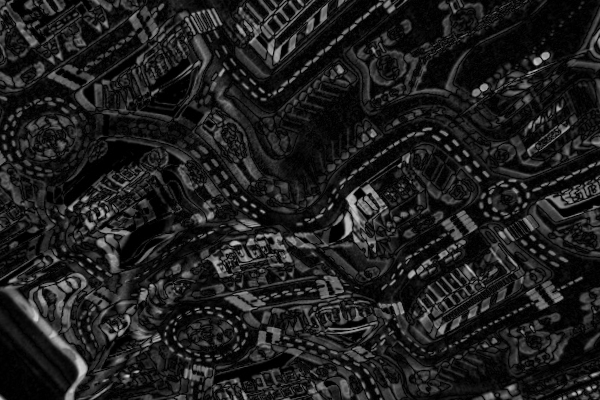
\includegraphics[width=\textwidth]{figures/rect_r2.jpg} 
    \caption{Right image (mean: 4.34).}
    \label{fig:rect_r2}
  \end{subfigure}
  \\
  \begin{subfigure}[b]{0.7\textwidth}
    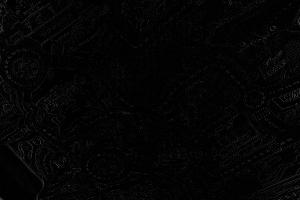
\includegraphics[width=\textwidth]{figures/rect_r2_transform.jpg} 
    \caption{Right image obtained with transformation (mean: 4.34).}
    \label{fig:rect_r2_transform}
  \end{subfigure}
  \caption{Rectification intensity errors $\Delta I_{i,j}$ with $n_x = 300$ and $n_y = 200$.}
\end{figure}

The photometric error in the original and rectified image are is shown in Figures
\ref{fig:rect_ru} and \ref{fig:rect_rw}. Since at this stage, no reliable depth
information is available, low photometric errors cannot be expected, which explains 
the relatively high average value. However, we know that the photometric errors should 
be approximately the same in the rectified and non-rectified images.
This behaviour is indeed observable, as shown by the difference image (Figure
\ref{fig:rect_rdiff}).

\begin{figure}[h]
  \centering
  \begin{subfigure}[b]{0.49\textwidth}
    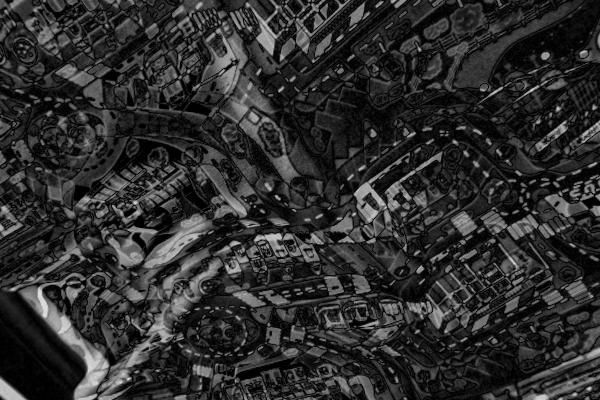
\includegraphics[width=\textwidth]{figures/rect_ru.jpg} 
    \caption{Original image (mean: 44.97).}
    \label{fig:rect_ru}
  \end{subfigure}
  \begin{subfigure}[b]{0.49\textwidth}
    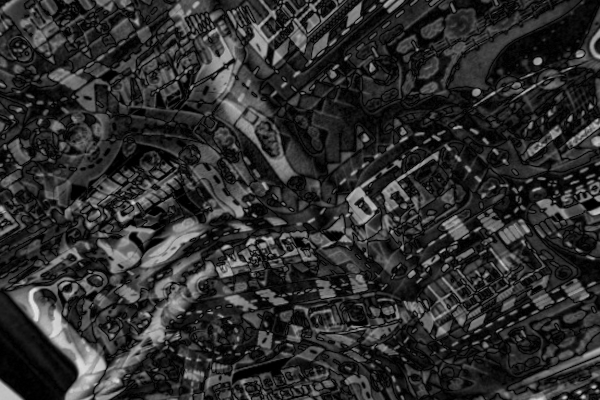
\includegraphics[width=\textwidth]{figures/rect_rw.jpg} 
    \caption{Rectified image (mean: 46.23).}
    \label{fig:rect_rw}
  \end{subfigure}
  \\
  \begin{subfigure}[b]{0.7\textwidth}
    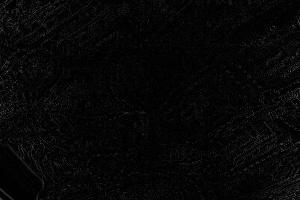
\includegraphics[width=\textwidth]{figures/rect_rdiff.jpg} 
    \caption{Difference of original and rectified image (mean: 6.71).}
    \label{fig:rect_rdiff}
  \end{subfigure}
  \caption{Rectification residual errors with $n_x = 300$ and $n_y = 200$.}
  \label{fig:rect}
\end{figure}

